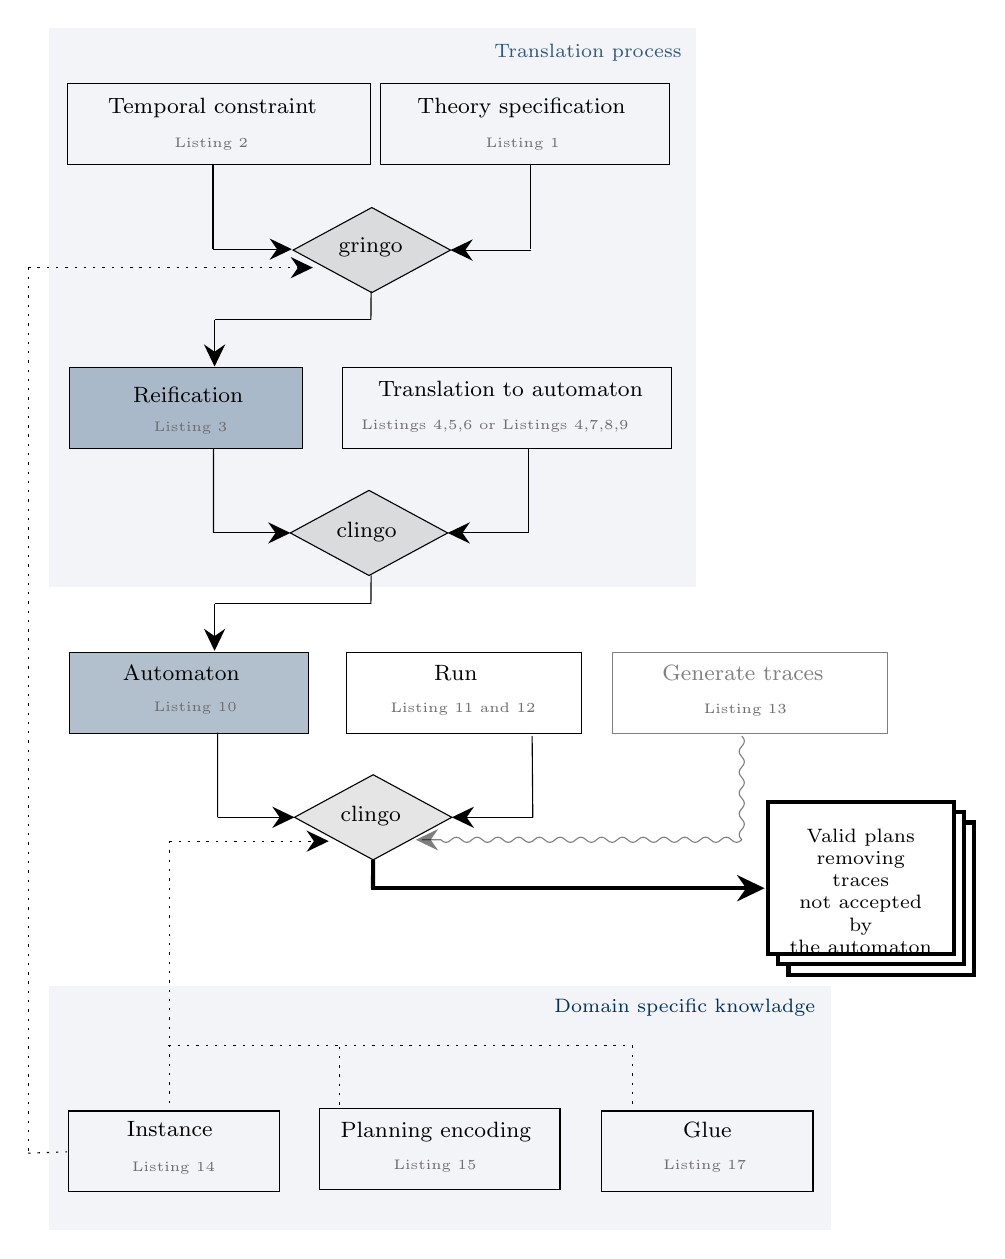
\begin{tikzpicture}[x=0.75pt,y=0.75pt,yscale=-1,xscale=1]
    %uncomment if require: \path (0,1205); %set diagram left start at 0, and has height of 1205
    
    %Shape: Rectangle [id:dp24788206372761257] 
    \draw  [fill={rgb, 255:red, 255; green, 255; blue, 255 }  ,fill opacity=1 ][line width=1.5]  (407,417) -- (496.55,417) -- (496.55,490.33) -- (407,490.33) -- cycle ;
    %Shape: Rectangle [id:dp28514107724578674] 
    \draw  [draw opacity=0][fill={rgb, 255:red, 0; green, 48; blue, 94 }  ,fill opacity=0.05 ][dash pattern={on 4.5pt off 4.5pt}] (50.5,495.67) -- (427.5,495.67) -- (427.5,613.33) -- (50.5,613.33) -- cycle ;
    %Shape: Rectangle [id:dp5077567162322292] 
    \draw  [draw opacity=0][fill={rgb, 255:red, 0; green, 48; blue, 94 }  ,fill opacity=0.05 ][dash pattern={on 4.5pt off 4.5pt}] (50.5,34.33) -- (362.5,34.33) -- (362.5,303.67) -- (50.5,303.67) -- cycle ;
    %Shape: Rectangle [id:dp8556117536304467] 
    \draw   (59.62,61) -- (205.42,61) -- (205.42,99.99) -- (59.62,99.99) -- cycle ;
    %Shape: Rectangle [id:dp3061835675075918] 
    \draw   (210.42,61) -- (349.62,61) -- (349.62,99.99) -- (210.42,99.99) -- cycle ;
    %Shape: Diamond [id:dp9415203890971041] 
    \draw  [fill={rgb, 255:red, 0; green, 0; blue, 0 }  ,fill opacity=0.1 ] (206.26,120.72) -- (244.17,141.22) -- (206.26,161.72) -- (168.34,141.22) -- cycle ;
    %Shape: Rectangle [id:dp0658574478056273] 
    \draw  [fill={rgb, 255:red, 0; green, 48; blue, 94 }  ,fill opacity=0.3 ] (60.62,198) -- (172.82,198) -- (172.82,236.99) -- (60.62,236.99) -- cycle ;
    %Shape: Rectangle [id:dp5420933852408244] 
    \draw   (192,198) -- (350.62,198) -- (350.62,236.99) -- (192,236.99) -- cycle ;
    %Shape: Diamond [id:dp7804185186549131] 
    \draw  [fill={rgb, 255:red, 0; green, 0; blue, 0 }  ,fill opacity=0.1 ] (204.91,257) -- (242.82,277.5) -- (204.91,298) -- (167,277.5) -- cycle ;
    %Shape: Rectangle [id:dp1579782039966966] 
    \draw  [fill={rgb, 255:red, 0; green, 48; blue, 94 }  ,fill opacity=0.3 ] (60.62,335) -- (175.82,335) -- (175.82,373.99) -- (60.62,373.99) -- cycle ;
    %Shape: Rectangle [id:dp21922696630916938] 
    \draw   (194,335) -- (307.15,335) -- (307.15,373.99) -- (194,373.99) -- cycle ;
    %Shape: Rectangle [id:dp26411591151258274] 
    \draw   (60,556) -- (161.82,556) -- (161.82,594.99) -- (60,594.99) -- cycle ;
    %Shape: Rectangle [id:dp9844105373777315] 
    \draw   (181,555) -- (296.93,555) -- (296.93,593.99) -- (181,593.99) -- cycle ;
    %Straight Lines [id:da9179998540863822] 
    \draw    (129.72,140.78) -- (164.72,140.78) ;
    \draw [shift={(167.72,140.78)}, rotate = 180] [fill={rgb, 255:red, 0; green, 0; blue, 0 }  ][line width=0.08]  [draw opacity=0] (10.72,-5.15) -- (0,0) -- (10.72,5.15) -- (7.12,0) -- cycle    ;
    %Straight Lines [id:da7912143421177068] 
    \draw    (283.17,141.22) -- (247.17,141.22) ;
    \draw [shift={(244.17,141.22)}, rotate = 360] [fill={rgb, 255:red, 0; green, 0; blue, 0 }  ][line width=0.08]  [draw opacity=0] (10.72,-5.15) -- (0,0) -- (10.72,5.15) -- (7.12,0) -- cycle    ;
    %Straight Lines [id:da8027967033545625] 
    \draw    (129.72,100.01) -- (129.72,140.78) ;
    %Straight Lines [id:da34160670813167726] 
    \draw    (282.72,100.01) -- (282.72,140.78) ;
    %Straight Lines [id:da568486742856372] 
    \draw    (205.83,174.67) -- (130.5,174.67) ;
    %Straight Lines [id:da9665051478374114] 
    \draw    (205.91,161) -- (205.83,174.67) ;
    %Straight Lines [id:da8317748002999547] 
    \draw    (281.82,277.5) -- (245.82,277.5) ;
    \draw [shift={(242.82,277.5)}, rotate = 360] [fill={rgb, 255:red, 0; green, 0; blue, 0 }  ][line width=0.08]  [draw opacity=0] (10.72,-5.15) -- (0,0) -- (10.72,5.15) -- (7.12,0) -- cycle    ;
    %Straight Lines [id:da4340309284116396] 
    \draw    (130,277.5) -- (164,277.5) ;
    \draw [shift={(167,277.5)}, rotate = 180] [fill={rgb, 255:red, 0; green, 0; blue, 0 }  ][line width=0.08]  [draw opacity=0] (10.72,-5.15) -- (0,0) -- (10.72,5.15) -- (7.12,0) -- cycle    ;
    %Straight Lines [id:da01308781139505788] 
    \draw    (129.99,236.73) -- (130,277.5) ;
    %Straight Lines [id:da018636812707615635] 
    \draw    (281.82,236.73) -- (281.82,277.5) ;
    %Straight Lines [id:da4867545297302681] 
    \draw  [dash pattern={on 0.84pt off 2.51pt}]  (108.72,426) -- (108.72,556.78) ;
    %Straight Lines [id:da3830532801993999] 
    \draw  [dash pattern={on 0.84pt off 2.51pt}]  (108.28,524.5) -- (332,524.5) ;
    %Straight Lines [id:da09223868766688892] 
    \draw  [dash pattern={on 0.84pt off 2.51pt}]  (190.5,525) -- (190.5,555.78) ;
    %Shape: Rectangle [id:dp5976304597228406] 
    \draw   (317,556) -- (418.82,556) -- (418.82,594.99) -- (317,594.99) -- cycle ;
    %Straight Lines [id:da4410590236065801] 
    \draw  [dash pattern={on 0.84pt off 2.51pt}]  (332,524.5) -- (332,556) ;
    %Straight Lines [id:da19225338333819464] 
    \draw  [dash pattern={on 0.84pt off 2.51pt}]  (40.72,149.67) -- (40.72,234) -- (40.72,576.33) ;
    %Straight Lines [id:da5024645482307678] 
    \draw  [dash pattern={on 0.84pt off 2.51pt}]  (40.72,149.67) -- (174.83,149.67) ;
    \draw [shift={(177.83,149.67)}, rotate = 180] [fill={rgb, 255:red, 0; green, 0; blue, 0 }  ][line width=0.08]  [draw opacity=0] (10.72,-5.15) -- (0,0) -- (10.72,5.15) -- (7.12,0) -- cycle    ;
    %Straight Lines [id:da5764659676991815] 
    \draw    (130.5,174.67) -- (130.5,194.33) ;
    \draw [shift={(130.5,197.33)}, rotate = 270] [fill={rgb, 255:red, 0; green, 0; blue, 0 }  ][line width=0.08]  [draw opacity=0] (10.72,-5.15) -- (0,0) -- (10.72,5.15) -- (7.12,0) -- cycle    ;
    %Straight Lines [id:da894604227602381] 
    \draw    (205.83,311.67) -- (130.5,311.67) ;
    %Straight Lines [id:da7188860332630708] 
    \draw    (130.5,311.67) -- (130.5,331.33) ;
    \draw [shift={(130.5,334.33)}, rotate = 270] [fill={rgb, 255:red, 0; green, 0; blue, 0 }  ][line width=0.08]  [draw opacity=0] (10.72,-5.15) -- (0,0) -- (10.72,5.15) -- (7.12,0) -- cycle    ;
    %Straight Lines [id:da3554509769994919] 
    \draw [line width=1.5]    (206.91,435) -- (206.83,448.67) ;
    %Straight Lines [id:da01324335735982407] 
    \draw  [dash pattern={on 0.84pt off 2.51pt}]  (40.72,576.33) -- (59.5,575.67) ;
    %Shape: Diamond [id:dp05782883080844736] 
    \draw  [fill={rgb, 255:red, 0; green, 0; blue, 0 }  ,fill opacity=0.1 ] (206.91,394) -- (244.82,414.5) -- (206.91,435) -- (169,414.5) -- cycle ;
    %Straight Lines [id:da09361882010550071] 
    \draw    (283.82,414.5) -- (247.82,414.5) ;
    \draw [shift={(244.82,414.5)}, rotate = 360] [fill={rgb, 255:red, 0; green, 0; blue, 0 }  ][line width=0.08]  [draw opacity=0] (10.72,-5.15) -- (0,0) -- (10.72,5.15) -- (7.12,0) -- cycle    ;
    %Straight Lines [id:da8326999325766362] 
    \draw    (132,414.5) -- (166,414.5) ;
    \draw [shift={(169,414.5)}, rotate = 180] [fill={rgb, 255:red, 0; green, 0; blue, 0 }  ][line width=0.08]  [draw opacity=0] (10.72,-5.15) -- (0,0) -- (10.72,5.15) -- (7.12,0) -- cycle    ;
    %Straight Lines [id:da35955432939448473] 
    \draw    (131.99,373.73) -- (132,414.5) ;
    %Straight Lines [id:da9796511600274105] 
    \draw    (283.5,375.33) -- (283.82,414.5) ;
    %Straight Lines [id:da08381943402202785] 
    \draw  [dash pattern={on 0.84pt off 2.51pt}]  (108.72,426) -- (182.5,426) ;
    \draw [shift={(185.5,426)}, rotate = 180] [fill={rgb, 255:red, 0; green, 0; blue, 0 }  ][line width=0.08]  [draw opacity=0] (10.72,-5.15) -- (0,0) -- (10.72,5.15) -- (7.12,0) -- cycle    ;
    %Straight Lines [id:da34272684140341236] 
    \draw [line width=1.5]    (391.5,448.67) -- (205.83,448.67) ;
    \draw [shift={(395.5,448.67)}, rotate = 180] [fill={rgb, 255:red, 0; green, 0; blue, 0 }  ][line width=0.08]  [draw opacity=0] (13.4,-6.43) -- (0,0) -- (13.4,6.44) -- (8.9,0) -- cycle    ;
    %Straight Lines [id:da38816660652930635] 
    \draw    (205.91,298) -- (205.83,311.67) ;
    %Shape: Rectangle [id:dp31370535660350696] 
    \draw  [color={rgb, 255:red, 0; green, 0; blue, 0 }  ,draw opacity=0.5 ] (322.15,335) -- (454.62,335) -- (454.62,373.99) -- (322.15,373.99) -- cycle ;
    %Straight Lines [id:da9731404355029183] 
    \draw [color={rgb, 255:red, 0; green, 0; blue, 0 }  ,draw opacity=0.5 ]   (384.5,375.33) .. controls (386.17,377) and (386.17,378.66) .. (384.5,380.33) .. controls (382.83,382) and (382.83,383.66) .. (384.5,385.33) .. controls (386.17,387) and (386.17,388.66) .. (384.5,390.33) .. controls (382.83,392) and (382.83,393.66) .. (384.5,395.33) .. controls (386.17,397) and (386.17,398.66) .. (384.5,400.33) .. controls (382.83,402) and (382.83,403.66) .. (384.5,405.33) .. controls (386.17,407) and (386.17,408.66) .. (384.5,410.33) .. controls (382.83,412) and (382.83,413.66) .. (384.5,415.33) .. controls (386.17,417) and (386.17,418.66) .. (384.5,420.33) .. controls (382.83,422) and (382.83,423.66) .. (384.5,425.33) -- (384.5,425.33) -- (384.5,425.33) ;
    %Straight Lines [id:da6224255621877544] 
    \draw [color={rgb, 255:red, 0; green, 0; blue, 0 }  ,draw opacity=0.5 ]   (384.5,425.33) .. controls (382.83,427) and (381.17,427) .. (379.5,425.33) .. controls (377.83,423.66) and (376.17,423.66) .. (374.5,425.33) .. controls (372.83,427) and (371.17,427) .. (369.5,425.33) .. controls (367.83,423.66) and (366.17,423.66) .. (364.5,425.33) .. controls (362.83,427) and (361.17,427) .. (359.5,425.33) .. controls (357.83,423.66) and (356.17,423.66) .. (354.5,425.33) .. controls (352.83,427) and (351.17,427) .. (349.5,425.33) .. controls (347.83,423.66) and (346.17,423.66) .. (344.5,425.33) .. controls (342.83,427) and (341.17,427) .. (339.5,425.33) .. controls (337.83,423.66) and (336.17,423.66) .. (334.5,425.33) .. controls (332.83,427) and (331.17,427) .. (329.5,425.33) .. controls (327.83,423.66) and (326.17,423.66) .. (324.5,425.33) .. controls (322.83,427) and (321.17,427) .. (319.5,425.33) .. controls (317.83,423.66) and (316.17,423.66) .. (314.5,425.33) .. controls (312.83,427) and (311.17,427) .. (309.5,425.33) .. controls (307.83,423.66) and (306.17,423.66) .. (304.5,425.33) .. controls (302.83,427) and (301.17,427) .. (299.5,425.33) .. controls (297.83,423.66) and (296.17,423.66) .. (294.5,425.33) .. controls (292.83,427) and (291.17,427) .. (289.5,425.33) .. controls (287.83,423.66) and (286.17,423.66) .. (284.5,425.33) .. controls (282.83,427) and (281.17,427) .. (279.5,425.33) .. controls (277.83,423.66) and (276.17,423.66) .. (274.5,425.33) .. controls (272.83,427) and (271.17,427) .. (269.5,425.33) .. controls (267.83,423.66) and (266.17,423.66) .. (264.5,425.33) .. controls (262.83,427) and (261.17,427) .. (259.5,425.33) .. controls (257.83,423.66) and (256.17,423.66) .. (254.5,425.33) .. controls (252.83,427) and (251.17,427) .. (249.5,425.33) .. controls (247.83,423.66) and (246.17,423.66) .. (244.5,425.33) .. controls (242.83,427) and (241.17,427) .. (239.5,425.33) -- (238.5,425.33) -- (230.5,425.33) ;
    \draw [shift={(227.5,425.33)}, rotate = 360] [fill={rgb, 255:red, 0; green, 0; blue, 0 }  ,fill opacity=0.5 ][line width=0.08]  [draw opacity=0] (10.72,-5.15) -- (0,0) -- (10.72,5.15) -- (7.12,0) -- cycle    ;
    %Shape: Rectangle [id:dp4398006989421265] 
    \draw  [fill={rgb, 255:red, 255; green, 255; blue, 255 }  ,fill opacity=1 ][line width=1.5]  (402,412) -- (491.55,412) -- (491.55,485.33) -- (402,485.33) -- cycle ;
    %Shape: Rectangle [id:dp7390603575053865] 
    \draw  [fill={rgb, 255:red, 255; green, 255; blue, 255 }  ,fill opacity=1 ][line width=1.5]  (397,407) -- (486.55,407) -- (486.55,480.33) -- (397,480.33) -- cycle ;
    
    % Text Node
    \draw (78,66.93) node [anchor=north west][inner sep=0.75pt]  [font=\footnotesize] [align=left] {Temporal constraint};
    % Text Node
    \draw (227,66.93) node [anchor=north west][inner sep=0.75pt]  [font=\footnotesize] [align=left] {Theory specification};
    % Text Node
    \draw (189,133.93) node [anchor=north west][inner sep=0.75pt]  [font=\footnotesize] [align=left] {gringo};
    % Text Node
    \draw (90,205.93) node [anchor=north west][inner sep=0.75pt]  [font=\footnotesize] [align=left] {Reification};
    % Text Node
    \draw (208,202.93) node [anchor=north west][inner sep=0.75pt]  [font=\footnotesize] [align=left] {Translation to automaton};
    % Text Node
    \draw (188,270.93) node [anchor=north west][inner sep=0.75pt]  [font=\footnotesize] [align=left] {clingo};
    % Text Node
    \draw (85,339.93) node [anchor=north west][inner sep=0.75pt]  [font=\footnotesize] [align=left] {Automaton};
    % Text Node
    \draw (235,339.93) node [anchor=north west][inner sep=0.75pt]  [font=\footnotesize] [align=left] {Run};
    % Text Node
    \draw (87,559.93) node [anchor=north west][inner sep=0.75pt]  [font=\footnotesize] [align=left] {Instance};
    % Text Node
    \draw (190,559.93) node [anchor=north west][inner sep=0.75pt]  [font=\footnotesize] [align=left] {Planning encoding};
    % Text Node
    \draw (404,418.93) node [anchor=north west][inner sep=0.75pt]  [font=\scriptsize] [align=left] {\begin{minipage}[lt]{54.78804595947266pt}\setlength\topsep{0pt}
    \begin{center}
    Valid plans\\removing traces\\not accepted by \\the automaton
    \end{center}
    
    \end{minipage}};
    % Text Node
    \draw (355,559.93) node [anchor=north west][inner sep=0.75pt]  [font=\footnotesize] [align=left] {Glue};
    % Text Node
    \draw (190,407.93) node [anchor=north west][inner sep=0.75pt]  [font=\footnotesize] [align=left] {clingo};
    % Text Node
    \draw (293,500.6) node [anchor=north west][inner sep=0.75pt]  [font=\scriptsize,color={rgb, 255:red, 0; green, 48; blue, 94 }  ,opacity=1 ] [align=left] {Domain specific knowladge};
    % Text Node
    \draw (264,40.6) node [anchor=north west][inner sep=0.75pt]  [font=\scriptsize,color={rgb, 255:red, 0; green, 48; blue, 94 }  ,opacity=0.8 ] [align=left] {Translation process};
    % Text Node
    \draw (345,339.93) node [anchor=north west][inner sep=0.75pt]  [font=\footnotesize,color={rgb, 255:red, 0; green, 0; blue, 0 }  ,opacity=0.5 ] [align=left] {Generate traces};
    % Text Node
    \draw (110,85.93) node [anchor=north west][inner sep=0.75pt]  [font=\tiny,color={rgb, 255:red, 110; green, 108; blue, 108 }  ,opacity=1 ] [align=left] {Listing 2};
    % Text Node
    \draw (260,85.93) node [anchor=north west][inner sep=0.75pt]  [font=\tiny,color={rgb, 255:red, 110; green, 108; blue, 108 }  ,opacity=1 ] [align=left] {Listing 1};
    % Text Node
    \draw (100,222.93) node [anchor=north west][inner sep=0.75pt]  [font=\tiny,color={rgb, 255:red, 110; green, 108; blue, 108 }  ,opacity=1 ] [align=left] {Listing 3};
    % Text Node
    \draw (100,357.93) node [anchor=north west][inner sep=0.75pt]  [font=\tiny,color={rgb, 255:red, 110; green, 108; blue, 108 }  ,opacity=1 ] [align=left] {Listing 10};
    % Text Node
    \draw (200,221.93) node [anchor=north west][inner sep=0.75pt]  [font=\tiny,color={rgb, 255:red, 110; green, 108; blue, 108 }  ,opacity=1 ] [align=left] {Listings 4,5,6 or Listings 4,7,8,9};
    % Text Node
    \draw (214,357.93) node [anchor=north west][inner sep=0.75pt]  [font=\tiny,color={rgb, 255:red, 110; green, 108; blue, 108 }  ,opacity=1 ] [align=left] {Listing 11 and 12};
    % Text Node
    \draw (365,358.93) node [anchor=north west][inner sep=0.75pt]  [font=\tiny,color={rgb, 255:red, 110; green, 108; blue, 108 }  ,opacity=1 ] [align=left] {Listing 13};
    % Text Node
    \draw (89.5,579.6) node [anchor=north west][inner sep=0.75pt]  [font=\tiny,color={rgb, 255:red, 110; green, 108; blue, 108 }  ,opacity=1 ] [align=left] {Listing 14};
    % Text Node
    \draw (215.5,578.6) node [anchor=north west][inner sep=0.75pt]  [font=\tiny,color={rgb, 255:red, 110; green, 108; blue, 108 }  ,opacity=1 ] [align=left] {Listing 15};
    % Text Node
    \draw (345.5,578.6) node [anchor=north west][inner sep=0.75pt]  [font=\tiny,color={rgb, 255:red, 110; green, 108; blue, 108 }  ,opacity=1 ] [align=left] {Listing 17};
    
    
    \end{tikzpicture}
    